\PassOptionsToPackage{unicode=true}{hyperref} % options for packages loaded elsewhere
\PassOptionsToPackage{hyphens}{url}
%
\documentclass[ignorenonframetext,]{beamer}
\usepackage{pgfpages}
\setbeamertemplate{caption}[numbered]
\setbeamertemplate{caption label separator}{: }
\setbeamercolor{caption name}{fg=normal text.fg}
\beamertemplatenavigationsymbolsempty
% Prevent slide breaks in the middle of a paragraph:
\widowpenalties 1 10000
\raggedbottom
\setbeamertemplate{part page}{
\centering
\begin{beamercolorbox}[sep=16pt,center]{part title}
  \usebeamerfont{part title}\insertpart\par
\end{beamercolorbox}
}
\setbeamertemplate{section page}{
\centering
\begin{beamercolorbox}[sep=12pt,center]{part title}
  \usebeamerfont{section title}\insertsection\par
\end{beamercolorbox}
}
\setbeamertemplate{subsection page}{
\centering
\begin{beamercolorbox}[sep=8pt,center]{part title}
  \usebeamerfont{subsection title}\insertsubsection\par
\end{beamercolorbox}
}
\AtBeginPart{
  \frame{\partpage}
}
\AtBeginSection{
  \ifbibliography
  \else
    \frame{\sectionpage}
  \fi
}
\AtBeginSubsection{
  \frame{\subsectionpage}
}
\usepackage{lmodern}
\usepackage{amssymb,amsmath}
\usepackage{ifxetex,ifluatex}
\usepackage{fixltx2e} % provides \textsubscript
\ifnum 0\ifxetex 1\fi\ifluatex 1\fi=0 % if pdftex
  \usepackage[T1]{fontenc}
  \usepackage[utf8]{inputenc}
  \usepackage{textcomp} % provides euro and other symbols
\else % if luatex or xelatex
  \usepackage{unicode-math}
  \defaultfontfeatures{Ligatures=TeX,Scale=MatchLowercase}
\fi
% use upquote if available, for straight quotes in verbatim environments
\IfFileExists{upquote.sty}{\usepackage{upquote}}{}
% use microtype if available
\IfFileExists{microtype.sty}{%
\usepackage[]{microtype}
\UseMicrotypeSet[protrusion]{basicmath} % disable protrusion for tt fonts
}{}
\IfFileExists{parskip.sty}{%
\usepackage{parskip}
}{% else
\setlength{\parindent}{0pt}
\setlength{\parskip}{6pt plus 2pt minus 1pt}
}
\usepackage{hyperref}
\hypersetup{
            pdftitle={Title},
            pdfauthor={J. J. Wannenburg},
            pdfborder={0 0 0},
            breaklinks=true}
\urlstyle{same}  % don't use monospace font for urls
\newif\ifbibliography
\usepackage{graphicx,grffile}
\makeatletter
\def\maxwidth{\ifdim\Gin@nat@width>\linewidth\linewidth\else\Gin@nat@width\fi}
\def\maxheight{\ifdim\Gin@nat@height>\textheight\textheight\else\Gin@nat@height\fi}
\makeatother
% Scale images if necessary, so that they will not overflow the page
% margins by default, and it is still possible to overwrite the defaults
% using explicit options in \includegraphics[width, height, ...]{}
\setkeys{Gin}{width=\maxwidth,height=\maxheight,keepaspectratio}
\setlength{\emergencystretch}{3em}  % prevent overfull lines
\providecommand{\tightlist}{%
  \setlength{\itemsep}{0pt}\setlength{\parskip}{0pt}}
\setcounter{secnumdepth}{0}

% set default figure placement to htbp
\makeatletter
\def\fps@figure{htbp}
\makeatother

\usepackage{tikz}

\makeatletter
\newbox\@backgroundblock
\newenvironment{backgroundblock}[2]{%
  \global\setbox\@backgroundblock=\vbox\bgroup%
    \unvbox\@backgroundblock%
    \vbox to0pt\bgroup\vskip#2\hbox to0pt\bgroup\hskip#1\relax%
}{\egroup\egroup\egroup}
\addtobeamertemplate{background}{\box\@backgroundblock}{}
\makeatother

\makeatletter
\setbeamertemplate{title page}{%
  \vbox{}
%  \vfill
  \begingroup
    \centering
    \begin{beamercolorbox}[sep=8pt,center]{title}
      \usebeamerfont{title}\inserttitle\par%
      \ifx\insertsubtitle\@empty%
      \else%
        \vskip0.25em%
        {\usebeamerfont{subtitle}\usebeamercolor[fg]{subtitle}\insertsubtitle\par}%
      \fi%     
    \end{beamercolorbox}%
    \vskip1em\par
    \begin{beamercolorbox}[sep=8pt,center]{author}
      \usebeamerfont{author}\insertauthor
    \end{beamercolorbox}
    \begin{beamercolorbox}[sep=8pt,center]{institute}
      \usebeamerfont{institute}\insertinstitute
    \end{beamercolorbox}
    \begin{beamercolorbox}[sep=5pt,center]{date}
      \usebeamerfont{date}\insertdate
    \end{beamercolorbox}%\vskip0.5em
    {\usebeamercolor[fg]{titlegraphic}\inserttitlegraphic\par}
  \endgroup
%  \vfill
}
\makeatother


\title{Title\thanks{This work was carried out within the project
\emph{Supporting the internationalization of the Institute of Computer
Science of the Czech Academy of Sciences}
(no.~CZ.02.2.69/0.0/0.0/18\_053/0017594), funded by the Operational
Programme Research, Development and Education of the Ministry of
Education, Youth and Sports of the Czech Republic. The project is
co-funded by the EU.}}
\providecommand{\subtitle}[1]{}
\subtitle{Conference Name}
\author{J. J. Wannenburg}
\providecommand{\institute}[1]{}
\institute{Institute of Computer Science, Academy of Sciences of the
Czech Republic, Czech Republic}
\date{Date}
\titlegraphic{\includegraphics{images/EUHorisontal.jpg}}

\begin{document}
\frame{\titlepage}

\begin{frame}{Test Animation}
\protect\hypertarget{test-animation}{}
When you arrive at the slide,

the animation is triggered

(unless you are in beamer)

\begin{itemize}
\tightlist
\item
  This is an itemized list
\item
  To the right is a lattice
\end{itemize}

\begin{enumerate}
[1)]
\tightlist
\item
  This is an enumerated list
\item
  Use arrows to move between slides
\item
  You can see the previous slide from the next slide
\end{enumerate}

\begin{backgroundblock}{0pt}{0pt}
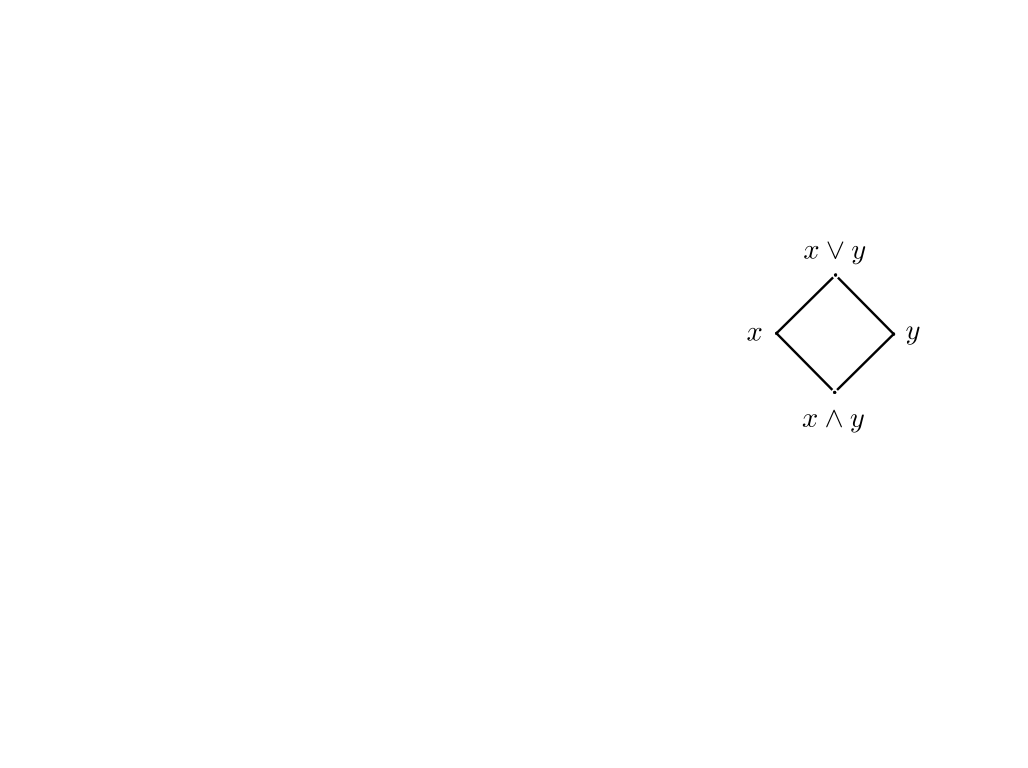
\includegraphics[keepaspectratio,width=\paperwidth]{images/LatticeOperations.pdf}
\end{backgroundblock}

\note{Some notes in \emph{markdown}.

One can create new lines as above to create space.

Slides start at the title of \# symbol and end at the dashes.

Note that beamer does not play the animation.}
\end{frame}

\begin{frame}{Environments}
\protect\hypertarget{environments}{}
\begin{description}
\tightlist
\item[Thm]
In the join of the six covers of \(\overline{\mathbf{C_4}}\) within
\(\mathsf{M}\), every subquasivariety is a variety.\\
~\\
\item[\(p, p \to q \vdash_{\mathbf{R^t}} q\)]
Suppose that \(e \leq p\) and \(e \leq p \to q\). By the law of
residuation \(p \leq q\), then \(e \leq q\), by the transitivity of
\(\leq\).\\
~\\
\end{description}

\begin{block}{Thm}
\protect\hypertarget{thm}{}
An alternative that goes with a proof

\begin{block}{Proof}
\protect\hypertarget{proof}{}
It is self evident.
\end{block}
\end{block}
\end{frame}

\begin{frame}{This slide has columns}
\protect\hypertarget{this-slide-has-columns}{}
\begin{columns}[T]
\begin{column}{0.48\textwidth}
left
\end{column}

\begin{column}{0.48\textwidth}
right
\end{column}
\end{columns}
\end{frame}

\begin{frame}{Using full-slide and columns}
\protect\hypertarget{using-full-slide-and-columns}{}
\begin{columns}[T]
\begin{column}{0.48\textwidth}
Recall that the Rieger-Nishimura lattice \(\mathbf{RN}\) is the
one-generated free Heyting algebra depicted below.
\end{column}

\begin{column}{0.48\textwidth}
\end{column}
\end{columns}

\begin{backgroundblock}{0pt}{0pt}
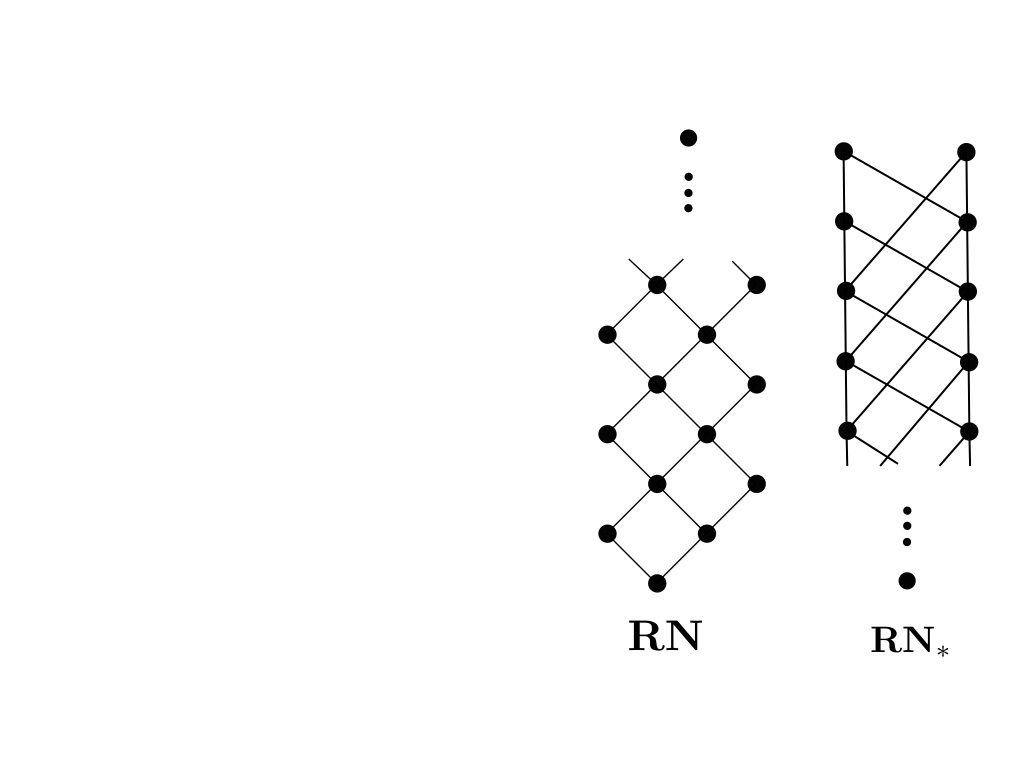
\includegraphics[keepaspectratio,width=\paperwidth]{images/RN.pdf}
\end{backgroundblock}
\end{frame}

\begin{frame}{Disappearing images}
\protect\hypertarget{disappearing-images}{}
\begin{backgroundblock}{0pt}{0pt}
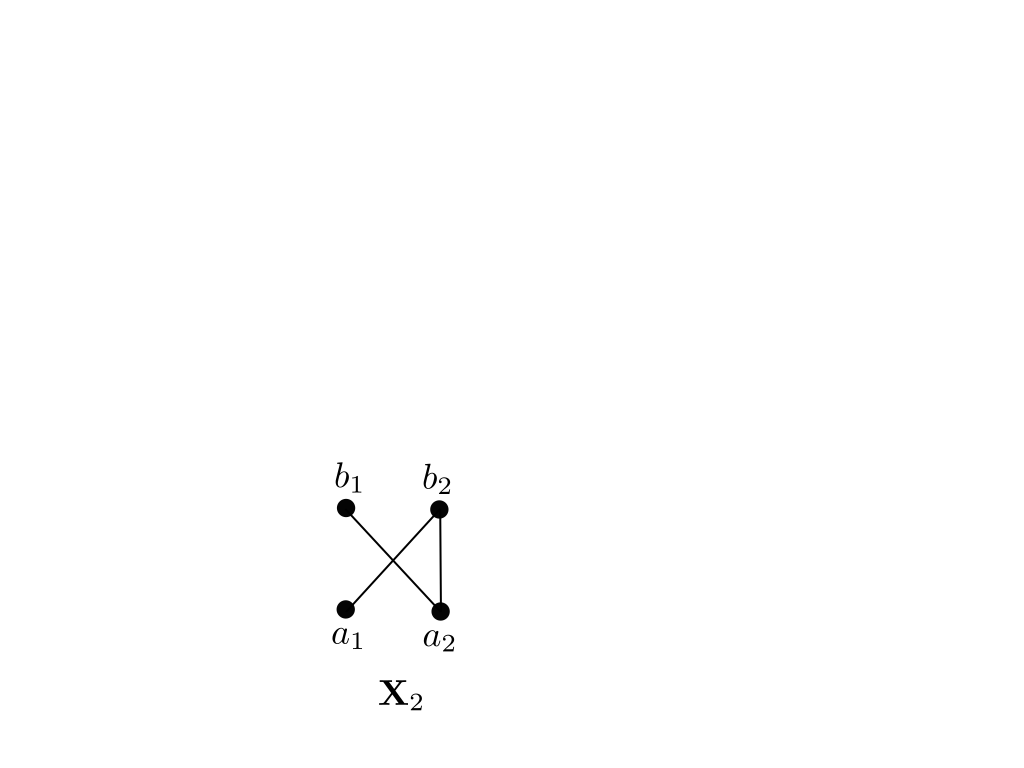
\includegraphics[keepaspectratio,width=\paperwidth]{images/Xn-1.pdf}
\end{backgroundblock}
\end{frame}

\begin{frame}{}
\protect\hypertarget{section}{}
\begin{backgroundblock}{0pt}{0pt}
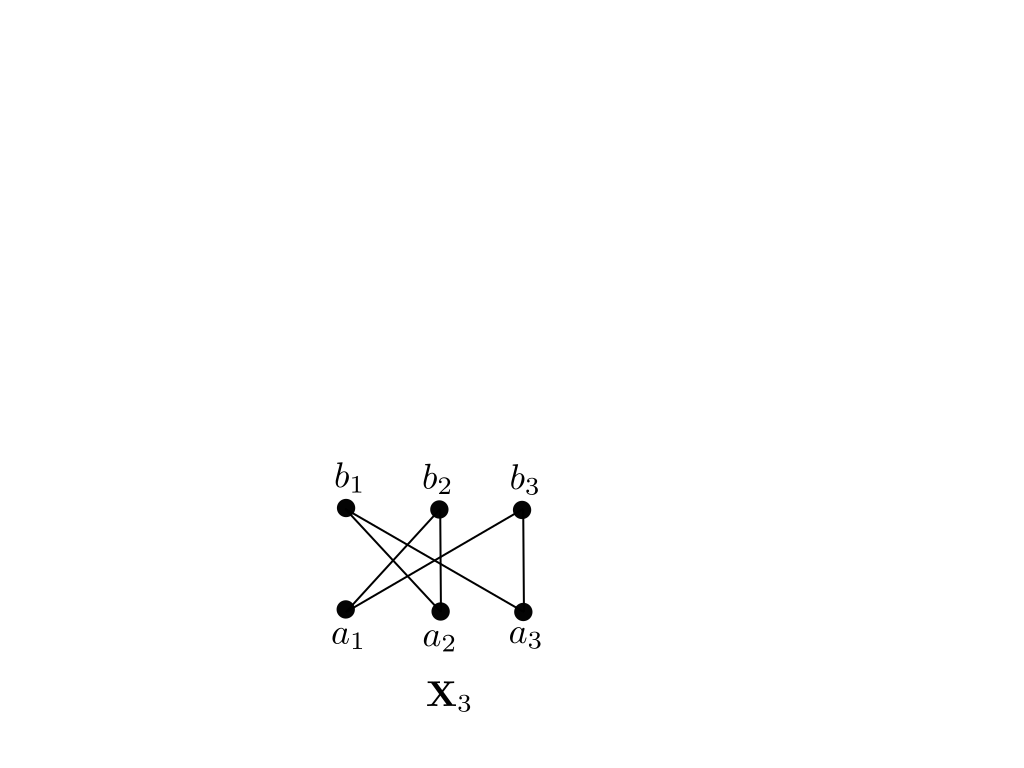
\includegraphics[keepaspectratio,width=\paperwidth]{images/Xn-2.pdf}
\end{backgroundblock}
\end{frame}

\begin{frame}{}
\protect\hypertarget{section-1}{}
\begin{backgroundblock}{0pt}{0pt}
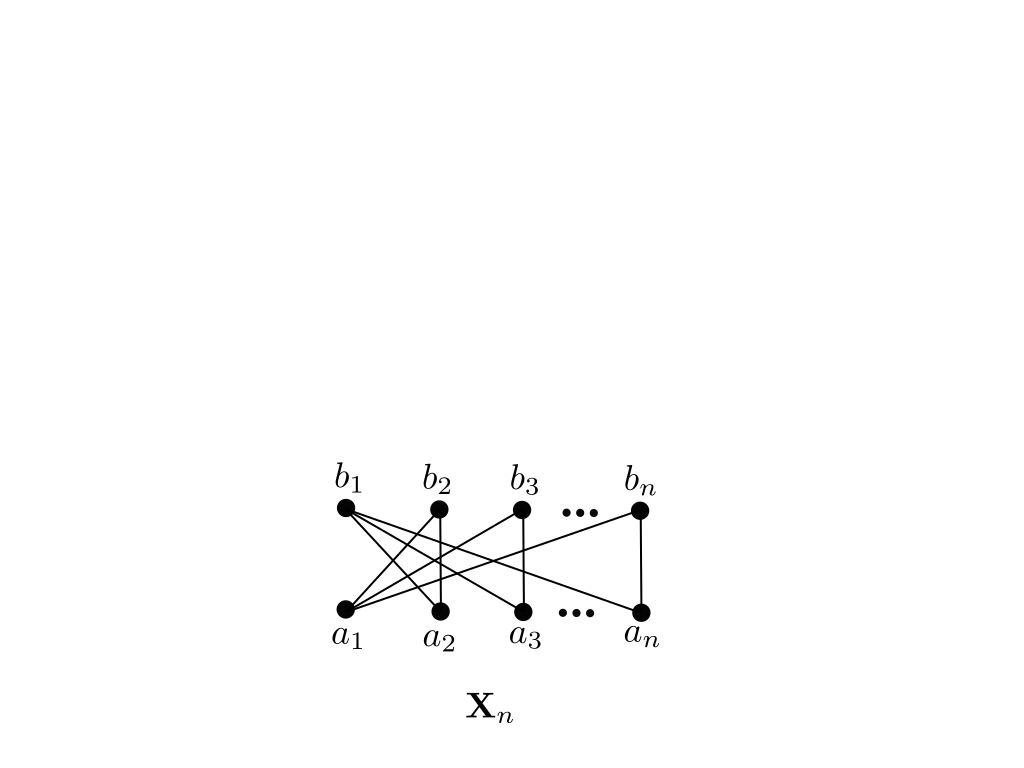
\includegraphics[keepaspectratio,width=\paperwidth]{images/Xn.pdf}
\end{backgroundblock}
\end{frame}

\begin{frame}{Fixed image}
\protect\hypertarget{fixed-image}{}
\begin{columns}[T]
\begin{column}{0.48\textwidth}
Keeping a `fixed' floating image.

Suppose this is a long proof.

And I want to keep the picture around as I continue with the proof.
\end{column}

\begin{column}{0.48\textwidth}
\end{column}
\end{columns}

\begin{backgroundblock}{0pt}{0pt}
\includegraphics[keepaspectratio,width=\paperwidth]{images/X2pinfty-epic-1.pdf}
\end{backgroundblock}
\end{frame}

\begin{frame}{}
\protect\hypertarget{section-2}{}
\begin{columns}[T]
\begin{column}{0.48\textwidth}
\hfill\break
\hfill\break
\hfill\break
\hfill\break

And do one more step.

And do one more step.

And do one more step.
\end{column}

\begin{column}{0.48\textwidth}
\end{column}
\end{columns}

\begin{backgroundblock}{0pt}{0pt}
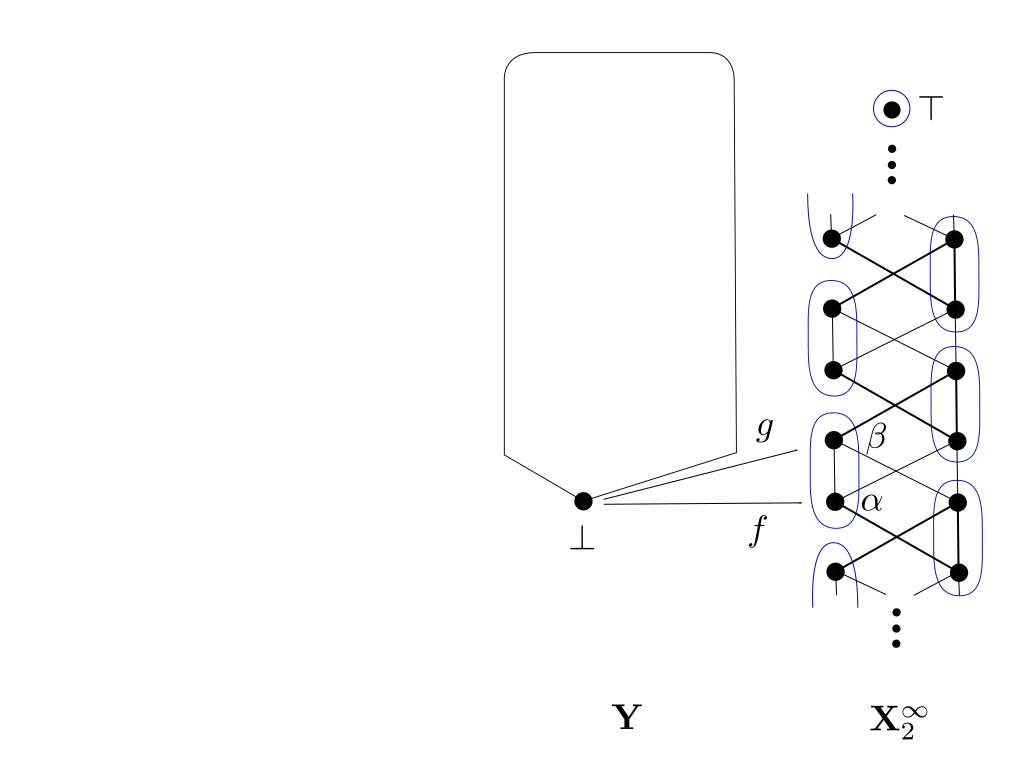
\includegraphics[keepaspectratio,width=\paperwidth]{images/X2pinfty-epic-2.pdf}
\end{backgroundblock}
\end{frame}

\begin{frame}{}
\protect\hypertarget{section-3}{}
\begin{columns}[T]
\begin{column}{0.48\textwidth}
\hfill\break
\hfill\break
\hfill\break
\hfill\break
\hfill\break
\hfill\break

And do one more step.

And do one more step.

And do one more step.
\end{column}

\begin{column}{0.48\textwidth}
\end{column}
\end{columns}

\begin{backgroundblock}{0pt}{0pt}
\includegraphics[keepaspectratio,width=\paperwidth]{images/X2pinfty-epic-3.pdf}
\end{backgroundblock}
\end{frame}

\begin{frame}{}
\protect\hypertarget{section-4}{}
\begin{columns}[T]
\begin{column}{0.48\textwidth}
\hfill\break
\hfill\break
\hfill\break
\hfill\break
\hfill\break
\hfill\break

And do one more step.

And do one more step.

And do one more step.
\end{column}

\begin{column}{0.48\textwidth}
\end{column}
\end{columns}

\begin{backgroundblock}{0pt}{0pt}
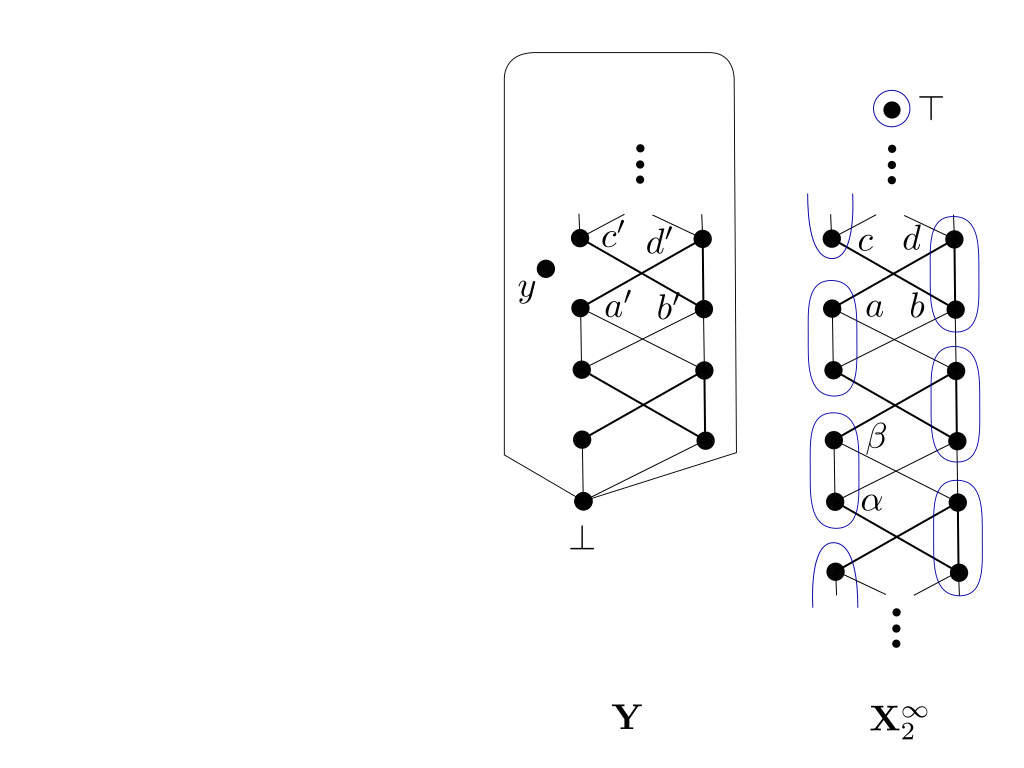
\includegraphics[keepaspectratio,width=\paperwidth]{images/X2pinfty-epic-4.pdf}
\end{backgroundblock}

\note{Note that creating frames in this way translates well to beamer.}
\end{frame}

\begin{frame}{}
\protect\hypertarget{section-5}{}
thank you
\end{frame}

\end{document}
